% Created 2024-05-30 jue 10:58
% Intended LaTeX compiler: pdflatex
\documentclass[a4paper]{article}
\usepackage[utf8]{inputenc}
\usepackage[T1]{fontenc}
\usepackage{graphicx}
\usepackage{longtable}
\usepackage{wrapfig}
\usepackage{rotating}
\usepackage[normalem]{ulem}
\usepackage{amsmath}
\usepackage{amssymb}
\usepackage{capt-of}
\usepackage{hyperref}
\usepackage[spanish]{babel}
\usepackage[usenames,dvipsnames]{color} % Required for custom colors
\renewcommand{\ttdefault}{pcr} % MONOESPACIO CON NEGRIT
\usepackage{lastpage}
\usepackage{listings}
\usepackage{listingsutf8}
\renewcommand{\lstlistingname}{Listado}
\lstset{frame=single,inputencoding=utf8,basicstyle=\scriptsize\ttfamily,showstringspaces=false,numbers=none}
\definecolor{MyDarkGreen}{rgb}{0.0,0.4,0.0} % This is the color used for comments
\lstset{ breaklines=true, postbreak=\mbox{\textcolor{red}{$\hookrightarrow$}\space}, keywordstyle=\bfseries, keywordstyle=[1]\color{Blue}\bfseries,  keywordstyle=[2]\color{Purple}\bfseries,  keywordstyle=[3]\color{Blue}\underbar,   identifierstyle=,   commentstyle=\usefont{T1}{pcr}{m}{sl}\color{MyDarkGreen}\small,   stringstyle=\color{Purple},   showstringspaces=false,   tabsize=2,   morecomment=[l][\color{Blue}]{...} }
\lstset{literate=  {á}{{\'a}}1 {é}{{\'e}}1 {í}{{\'i}}1 {ó}{{\'o}}1 {ú}{{\'u}}1   {Á}{{\'A}}1 {É}{{\'E}}1 {Í}{{\'I}}1 {Ó}{{\'O}}1 {Ú}{{\'U}}1   {à}{{\`a}}1 {è}{{\`e}}1 {ì}{{\`i}}1 {ò}{{\`o}}1 {ù}{{\`u}}1   {À}{{\`A}}1 {È}{{\'E}}1 {Ì}{{\`I}}1 {Ò}{{\`O}}1 {Ù}{{\`U}}1   {ä}{{\"a}}1 {ë}{{\"e}}1 {ï}{{\"i}}1 {ö}{{\"o}}1 {ü}{{\"u}}1   {Ä}{{\"A}}1 {Ë}{{\"E}}1 {Ï}{{\"I}}1 {Ö}{{\"O}}1 {Ü}{{\"U}}1   {â}{{\^a}}1 {ê}{{\^e}}1 {î}{{\^i}}1 {ô}{{\^o}}1 {û}{{\^u}}1   {Â}{{\^A}}1 {Ê}{{\^E}}1 {Î}{{\^I}}1 {Ô}{{\^O}}1 {Û}{{\^U}}1   {œ}{{\oe}}1 {Œ}{{\OE}}1 {æ}{{\ae}}1 {Æ}{{\AE}}1 {ß}{{\ss}}1   {ű}{{\H{u}}}1 {Ű}{{\H{U}}}1 {ő}{{\H{o}}}1 {Ő}{{\H{O}}}1   {ç}{{\c c}}1 {Ç}{{\c C}}1 {ø}{{\o}}1 {å}{{\r a}}1 {Å}{{\r A}}1   {€}{{\euro}}1 {£}{{\pounds}}1 {«}{{\guillemotleft}}1   {»}{{\guillemotright}}1 {ñ}{{\~n}}1 {Ñ}{{\~N}}1 {¿}{{?`}}1 }
\usepackage{caption}
\usepackage{attachfile2}
\usepackage[margin=1.5cm,includeheadfoot,includehead,includefoot]{geometry}
\hypersetup{colorlinks,linkcolor=black}
\usepackage{fancyhdr}
\pagestyle{fancyplain}
\chead{}
\lhead{}
\rhead{}
\cfoot{}
\lfoot{\begin{footnotesize}alvaro.gonzalezsotillo@educa.madrid.org\end{footnotesize}}
\rfoot{\begin{footnotesize}\thepage / \pageref{LastPage}\end{footnotesize}}
\usepackage[skins]{tcolorbox}
\usepackage{multicol}
\usepackage{changepage} %ajdustwidth
\usepackage{fancybox}
\usepackage{attachfile2}
\lhead{Extraordinaria 2021 (es el \\lhead)}
\rhead{Administración y Gestión de Bases de Datos (es el \\rhead)}
\lhead{Base de datos distribuida}
\rhead{Gestión de bases de datos}
\usepackage{svg}
\usepackage{letltxmacro}
\LetLtxMacro{\originalincludegraphics}{\includegraphics}
\renewcommand{\includegraphics}[2][]{\IfFileExists{#2.pdf}{\originalincludegraphics[#1]{#2.pdf}}{\originalincludegraphics[#1]{#2}}}
\LetLtxMacro{\originalincludesvg}{\includesvg}
\renewcommand{\includesvg}[2][]{\IfFileExists{#2.pdf}{\originalincludegraphics[#1]{#2.pdf}}{\originalincludegraphics[#1]{#2.svg.pdf}}}
\usepackage{comment}
\excludecomment{NOTES}
\author{Álvaro González Sotillo}
\date{\today}
\title{Práctica con empresas y sucursales}
\hypersetup{
 pdfauthor={Álvaro González Sotillo},
 pdftitle={Práctica con empresas y sucursales},
 pdfkeywords={},
 pdfsubject={},
 pdfcreator={Emacs 29.3 (Org mode 9.6.15)}, 
 pdflang={Spanish}}
\begin{document}

\maketitle
\setcounter{tocdepth}{1}
\tableofcontents

\captionsetup{font=scriptsize}

\setlength{\parindent}{0em}
\setlength{\parskip}{1em}

\newtcolorbox{Aviso}[1][Aviso]{
  enhanced,
  colback=gray!5!white,
  colframe=gray!75!black,fonttitle=\bfseries,
  colbacktitle=gray!85!black,
  attach boxed title to top left={yshift=-2mm,xshift=2mm},
  title=#1
}

\newtcolorbox{cuadrito}[1][Ignorado]{
  %drop shadow southeast,
  enhanced jigsaw,
  colback=white,
}


\newcommand{\StudentData}{
  \begin{cuadrito}[1\textwidth]
    \vspace{0.3cm}
    \large{
      \textbf{Apellidos:} \hrulefill \\
      \textbf{Nombre:} \hrulefill \\
      \textbf{Fecha:} \hrulefill \hspace{1cm} \textbf{Usuario:} \hrulefill \\
    }
    \vspace{-0.2cm}
  \end{cuadrito}
}



\section{Objetivo de la práctica}
\label{sec:org0000000}
En esta práctica el alumno utilizará la funcionalidad \emph{dblink} de Oracle para implementar una base de datos distribuida.



\section{Descripción del problema}
\label{sec:org0000003}
Cada alumno representará la sucursal de una empresa. La central de la empresa se representa por la base de datos del profesor.

Se desea que las dos bases de datos funcionen de forma distribuida sin replicación. Los datos se guardarán en la base de datos de la sede central o de la sucursal, pero podrán consultarse desde cualquiera de ellas.

Se utilizará como central el usuario del alumno en el servidor de clase (10.1.33.201). Cada alumno configurará una base de datos en su ordenador con los datos en la hoja de cálculo en \url{https://bit.ly/4bDtWdE}

Habrá una lista de clientes, de los que se conocerá un identificador y su nombre.

\newpage
\section{Vistas/tablas necesarias}
\label{sec:org000000f}
\subsection{Vistas/tablas/sinónimos en la sucursal}
\label{sec:org0000006}
\begin{itemize}
\item \texttt{T\_SUC\_CLIENTES(idcliente,nombrecliente)}: Debe ser una \textbf{tabla} almacenada en la sucursal, con la lista de clientes de la sucursal
\item \texttt{SUC\_CLIENTES(idcliente,nombrecliente)}: Lista de clientes dados de alta en la sucursal. Puede ser una tabla, una vista o un sinónimo.
\end{itemize}

\subsection{Vistas/tablas/sinónimos en la central}
\label{sec:org0000009}
\begin{itemize}
\item \texttt{T\_CEN\_CLIENTES(idcliente,nombrecliente)}: Debe ser una \textbf{tabla} almacenada en la central, con la lista de clientes de la central
\item \texttt{CEN\_CLIENTES(idcliente,nombrecliente)}: Lista de clientes dados de alta en la sucursal. Puede ser una tabla, una vista o un sinónimo.
\end{itemize}

\subsection{Vistas/sinónimos en la sucursal y en la central}
\label{sec:org000000c}
Estas vistas se definen en las dos bases de datos, y agrupan datos de la central y la sucursal
\begin{itemize}
\item \texttt{TODOS\_CLIENTES(localizacion,idcliente,nombrecliente)}: Lista de clientes dados de alta en la sucursal. Puede ser una tabla, una vista o un sinónimo.
\end{itemize}


\begin{center}
\begin{tabular}{lll}
Campo & tipo & \\[0pt]
\hline
\texttt{idcliente} & \texttt{NUMBER(10)} & El identificador de cliente\\[0pt]
\texttt{nombrecliente} & \texttt{VARCHAR(255)} & El nombre del cliente, que puede repetirse\\[0pt]
\texttt{localizacion} & \texttt{CHAR(1)} & \texttt{C} o \texttt{S}, para central o sucursal\\[0pt]
\end{tabular}
\end{center}


\newpage
<<<<<<< HEAD
\section{Creación de clientes (4 puntos)}
\label{sec:org0000012}
\texttt{=====}
\section{Creación de clientes}
\label{sec:org0000015}
>>>>>>> 0b7bad232eed818a0f3793b3bdd8ba981a929fe8
Los clientes se crearán realizando inserciones en \texttt{SUC\_CLIENTES} y \texttt{CEN\_CLIENTES}
\begin{itemize}
\item Las inserciones que especifiquen el \texttt{idcliente} provocarán el error \texttt{'SOBRANDATOS'}
\item El \texttt{idcliente} se extraerá de una secuencia. La secuencia será común para \texttt{SUC\_CLIENTES} y \texttt{CEN\_CLIENTES}. Esto quiere decir que el \texttt{idcliente} es único en toda la empresa.
\end{itemize}
También se pueden crear clientes insertando en \texttt{TODOS\_CLIENTES}
\begin{itemize}
\item El campo \texttt{localización} indicará si el cliente se almacena realmente en \texttt{SUC\_CLIENTES} o en \texttt{CEN\_CLIENTES}
\item Por lo demás, igual que el caso anterior
\end{itemize}



\begin{lstlisting}[language=SQL,label= ,caption={Sentencias de ejemplo en la sucursal},captionpos=b,numbers=none]
-- PROVOCA UN ERROR 'SOBRANDATOS'
insert into SUC_CLIENTES(idcliente,nombrecliente) values (1,'Un cliente');

-- INSERTA UN CLIENTE EN LA SUCURSAL
insert into SUC_CLIENTES(nombrecliente) values ('Un cliente');

-- INSERTA OTRO CLIENTE EN LA SUCURSAL
insert into TODOS_CLIENTES(nombrecliente,localizacion) values ('Otro cliente','S');

-- INSERTA OTRO CLIENTE EN LA CENTRAL
insert into TODOS_CLIENTES(nombrecliente,localizacion) values ('Otro cliente más','C');

select * from SUC_CLIENTES;
IDCLIENTE  NOMBRECLIENTE
---------  -------------
10         Un cliente
11         Otro cliente

select * from TODOS_CLIENTES;
IDCLIENTE  NOMBRECLIENTE     LOCALIZACION
---------  ----------------  ------------
10         Un cliente        S
11         Otro cliente      S
12         Otro cliente más  C
\end{lstlisting}

\begin{lstlisting}[language=SQL,label= ,caption={Sentencias de ejemplo en la central, tras las anteriores},captionpos=b,numbers=none]
-- PROVOCA UN ERROR 'SOBRANDATOS'
insert into CEN_CLIENTES(idcliente,nombrecliente) values (1,'A client');

-- INSERTA UN CLIENTE EN LA CENTRAL
insert into CEN_CLIENTES(nombrecliente) values ('A client');

-- INSERTA OTRO CLIENTE EN LA SUCURSAL
insert into TODOS_CLIENTES(nombrecliente,localizacion) values ('Another client','S');

-- INSERTA OTRO CLIENTE EN LA CENTRAL
insert into TODOS_CLIENTES(nombrecliente,localizacion) values ('Yet another client','C');

select * from CEN_CLIENTES;
IDCLIENTE  NOMBRECLIENTE
---------  -------------
12         Oro cliente más
13         A client
15         Yet another client

select * from TODOS_CLIENTES;
IDCLIENTE  NOMBRECLIENTE       LOCALIZACION
---------  ----------------    ------------
10         Un cliente          S
11         Otro cliente        S
12         Otro cliente más    C
13         A client            C
14         Another client      S
15         Yet another client  C
\end{lstlisting}

\section{Modificación de clientes (4 puntos)}
\label{sec:org0000018}
Se podrán ejecutar sentencias \texttt{UPDATE} sobre la vista \texttt{TODOS\_CLIENTES}
\begin{itemize}
\item Si se intenta modificar el campo \texttt{idcliente} o \texttt{nombrecliente} se producirá el error \texttt{'INMUTABLE'}.
\item Si se modifica el campo \texttt{localizacion}
\begin{itemize}
\item Si se cambia a \texttt{'C'} , el cliente se moverá de \texttt{T\_SUC\_CLIENTES} a \texttt{T\_CEN\_CLIENTES}
\item Si se cambia a \texttt{'S'} , el cliente se moverá de \texttt{T\_CEN\_CLIENTES} a \texttt{T\_SUC\_CLIENTES}
\end{itemize}
\end{itemize}

\begin{Aviso}
\texttt{TODOS\_CLIENTES} existe tanto en el servidor del profesor (central)  como en el del alumno (sucursal). Debe implementarse la funcionalidad en los dos servidores.
\end{Aviso}

\section{Borrado de clientes (2 puntos)}
\label{sec:org000001b}
Se podrán ejecutar sentencias \texttt{DELETE} sobre la vista \texttt{TODOS\_CLIENTES}
\begin{itemize}
\item Se borrará la entrada correspondiente teniendo en cuenta el campo \texttt{localizacion}, para saber si se borra de la sucursal o de la central.
\end{itemize}

\section{Instrucciones de entrega}
\label{sec:org000001e}
La autoría del trabajo es individual. Se corregirá \emph{on-line}, ejecutando pruebas mediante conexiones de red. Los servidores Oracle deberán estar funcionando y conectados en el día que el profesor pase dichas pruebas.

\section{Estrategia de implementación}
\label{sec:org0000021}
Hay varias opciones para implementar los requisitos de la práctica. Los siguientes diagramas indican dos posibilidades:


\begin{center}
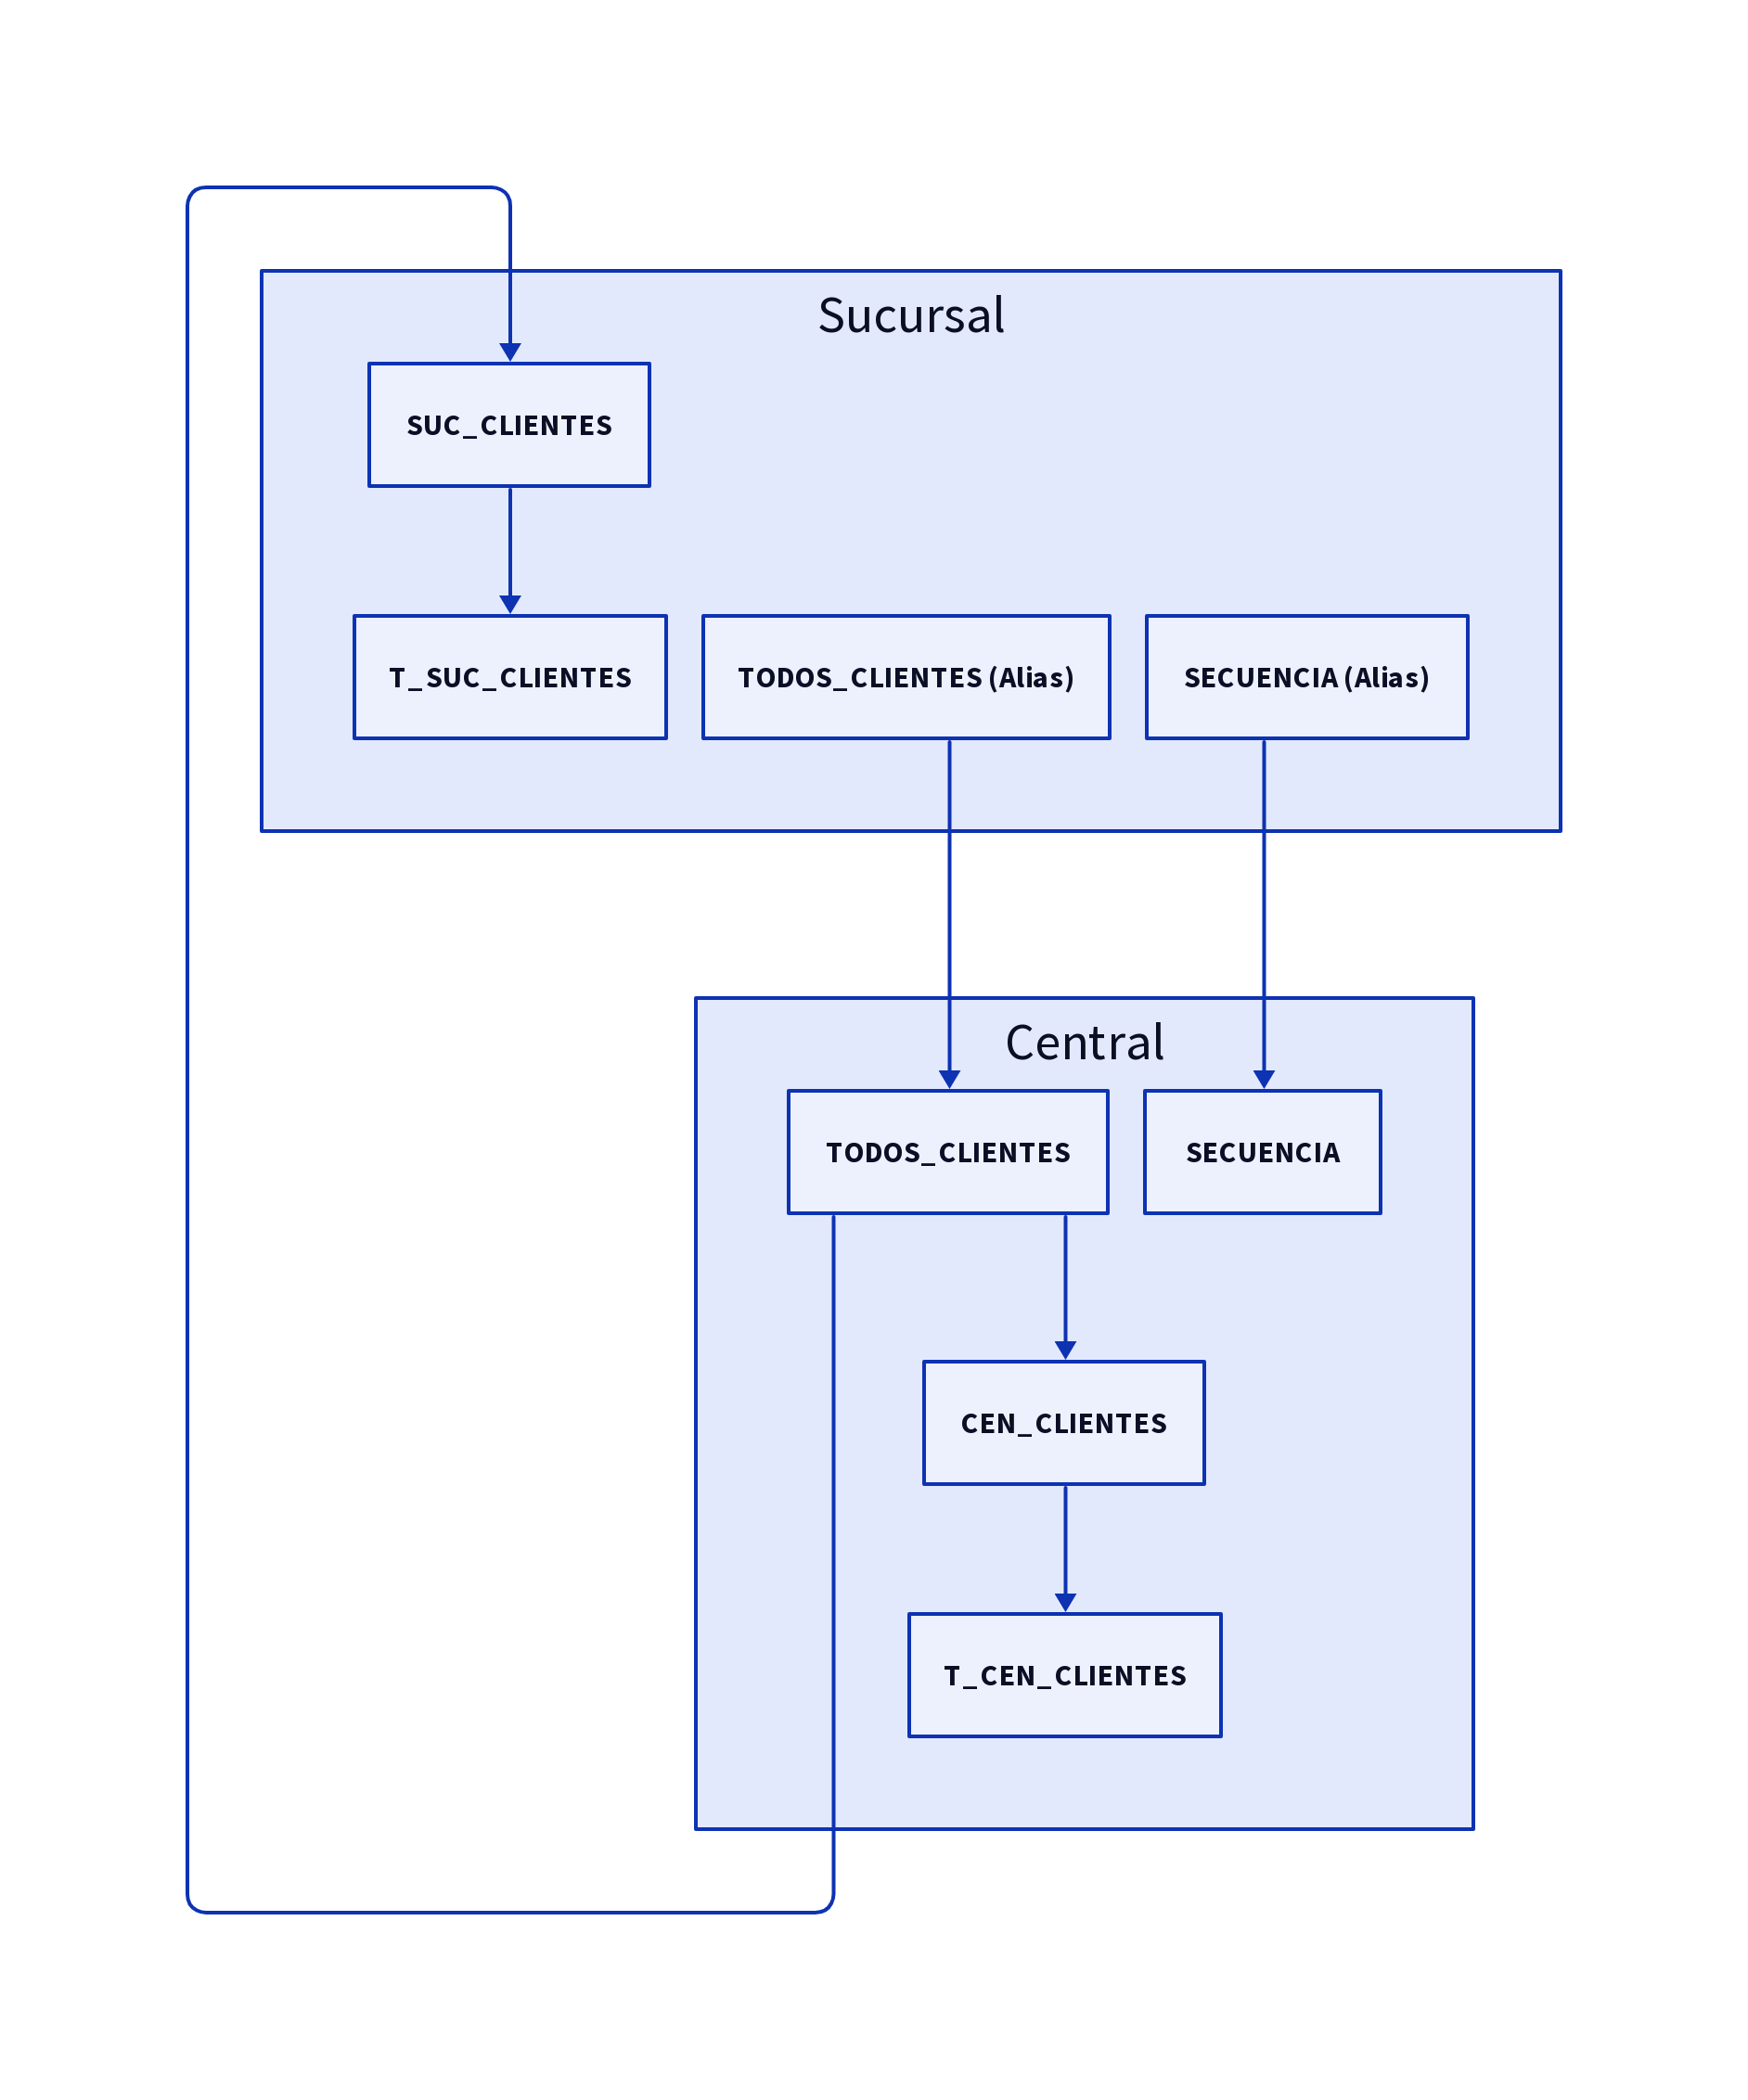
\includegraphics[width=.9\linewidth]{./dblinks-opcion-recomendada.png}
\end{center}


\begin{center}
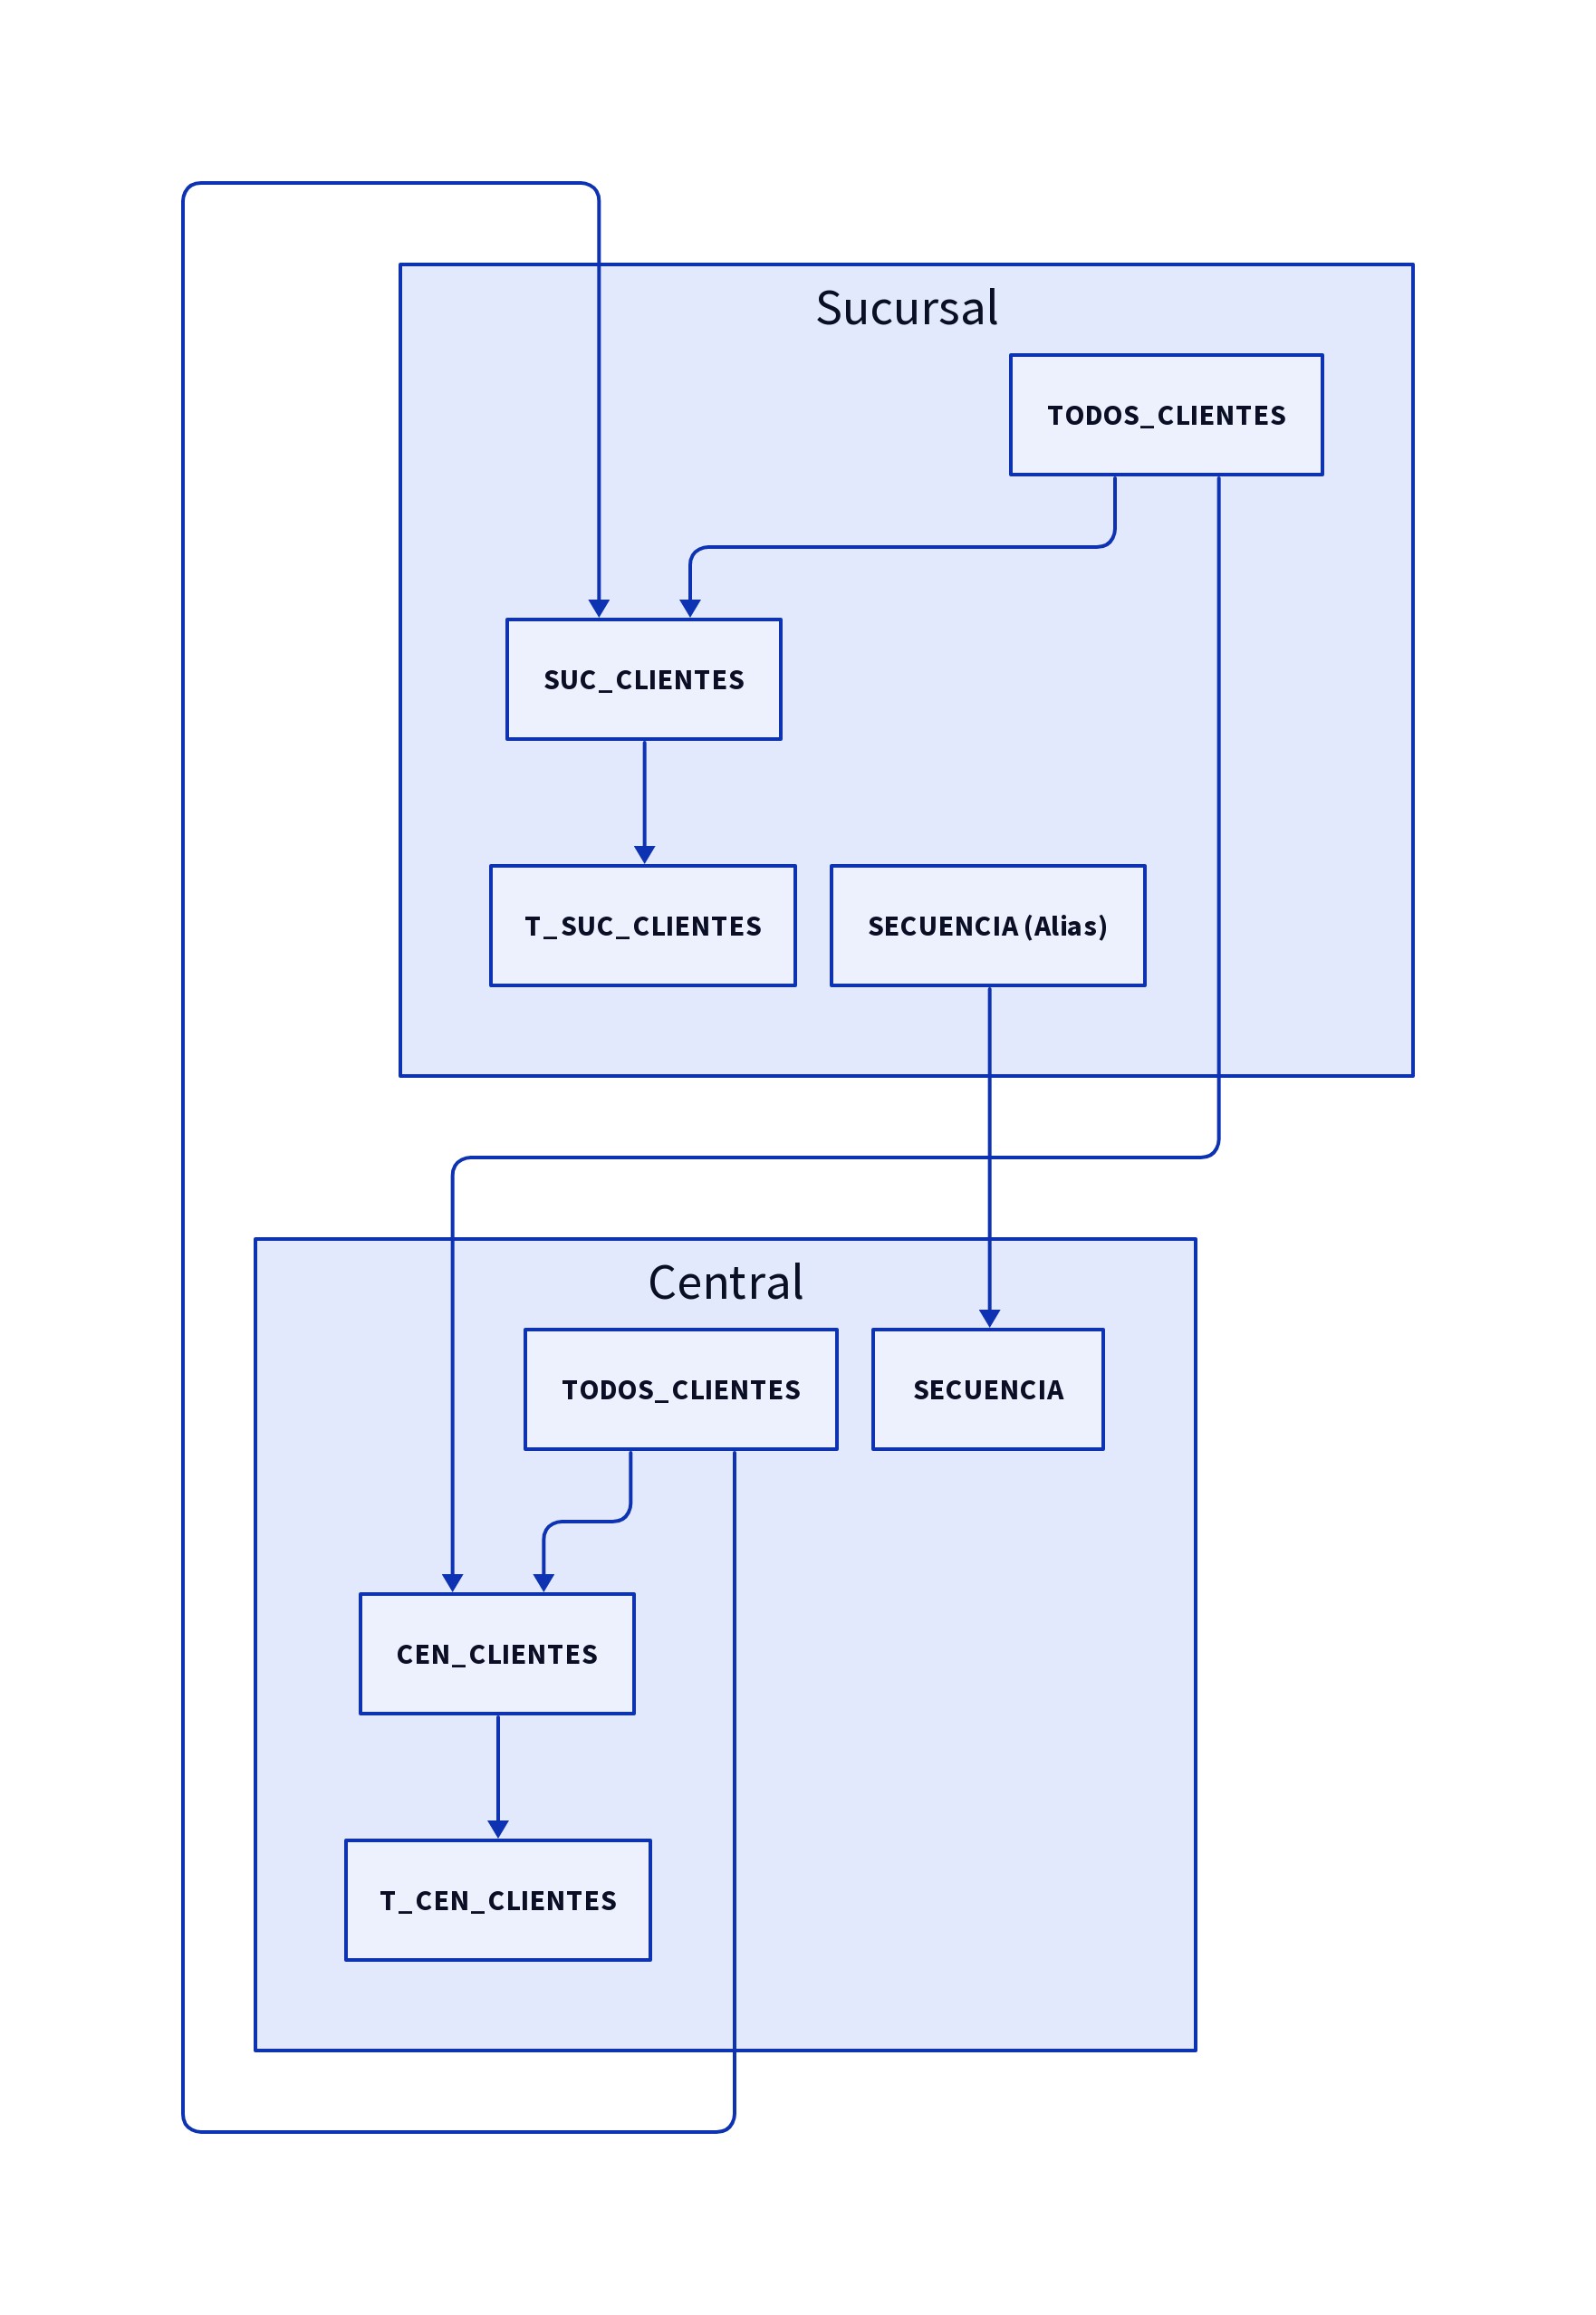
\includegraphics[width=.9\linewidth]{./dblinks-opcion-alternativa.png}
\end{center}
\end{document}
